\documentclass[12pt,a4paper]{article}
\usepackage[utf8]{inputenc}
\usepackage[T2A]{fontenc}
\usepackage[russian]{babel}
\usepackage{amsmath, amssymb, amsthm}
\usepackage[margin=2cm]{geometry}
\usepackage{hyperref}
\usepackage{enumitem}
\usepackage{booktabs}
\usepackage{xcolor}
\usepackage{graphicx} % Добавлен пакет для отображения картинок

\hypersetup{
    colorlinks=true,
    linkcolor=blue,
    urlcolor=blue,
    citecolor=purple % Изменено с black на purple для выделения цифр ссылок фиолетовым
}


\begin{document}

% Заголовок
\begin{center}
    \LARGE \bfseries
    Анализ робастности неявного градиентного \\
    спуска в архитектуре Transformer к выбросам \\
    (Outliers)
\end{center}

\vspace{0.8cm}

% Блок авторов
\begin{center}
    \begin{tabular}{cc}
        \large Владимир Назаров & \large Игнат Чернышов \\
        \texttt{nazarov.vr@phystech.edu} & \texttt{chernyshov.im@phystech.edu} \\
        \rule{0pt}{4ex} % Отступ между строками
        \large Марк Захаров & \large Максим Савичев \\
        \texttt{zakharov.mark@phystech.edu} & \texttt{savichev.mv@phystech.edu}
    \end{tabular}
\end{center}

\begin{center}
    \normalsize\href{https://github.com/MIPT-AI360-OPT-TEAM/AnalysisTransformersGD}{Репозиторий проекта: MIPT-AI360-OPT-TEAM/AnalysisTransformersGD}
\end{center}

\vspace{0.8cm}

% Дата
\begin{center}
    \large April 26, 2026
\end{center}

\vspace{1cm}


\section*{Executive Summary}
Данный документ представляет собой детальный план учебно-исследовательского проекта, направленного на изучение робастности In-Context Learning (ICL) в архитектурах Transformer. Основной вывод, который планируется получить: математически верифицировать способность трансформеров с нелинейностями (Softmax, MLP (Multi-Layer Perceptron)) переходить от симуляции градиентного спуска по уязвимой метрике MSE к робастным стратегиям оптимизации (например, аналогам функции потерь Хьюбера). Ожидаемые ключевые данные включают: точное совпадение извлеченных скрытых весов с аналитическими траекториями (оцениваемые через метрики $L_2$ Trajectory Proximity и Cosine Similarity), а также количественную оценку деградации на чистых данных (OOD Degradation Gap). Основные логистические рекомендации по выполнению проекта: использовать фреймворк PyTorch для преодоления устаревших зависимостей JAX, применять метод зондирования (weight probing) для прямой экстракции матриц и внедрить последовательный пайплайн экспериментов (от простейшего линейного внимания до полных слоев), что обеспечит строгое выполнение плана в отведенный 4-недельный срок.

\section*{Аннотация (Abstract)}
Современные исследования \cite{vonOswald2023} показывают, что прямой проход архитектуры Transformer способен аппроксимировать шаги градиентного спуска (GD). Данный учебно-исследовательский проект направлен на изучение границ применимости этого феномена в условиях зашумленных данных. Мы проверяем гипотезу о том, что при наличии экстремальных выбросов (outliers) в контексте, добавление нелинейностей (Softmax, MLP) позволяет модели эволюционировать от уязвимого метода наименьших квадратов (MSE) к робастным алгоритмам оптимизации. Путем извлечения скрытых весов трансформера методом зондирования (probing) и сопоставления их с аналитическими траекториями (MSE GD, Huber GD), проект переводит анализ In-Context Learning (ICL) из плоскости эмпирических наблюдений в область строгой математической верификации.

\section{Описание проекта и решаемая задача}
Проект является исследовательским расширением базовых работ по механистической интерпретации In-Context Learning \cite{vonOswald2023, garg2022what, akyurek2023what}. В классической задаче линейной регрессии модель обучается симулировать шаги градиентного спуска для минимизации среднеквадратичной ошибки (MSE):
\begin{equation}
    \min_\theta \frac{1}{n} \sum_{i=1}^n (x_i^T \theta - y_i)^2
\end{equation}
Однако классический градиентный спуск по MSE имеет фундаментальный математический недостаток: он крайне чувствителен к выбросам, так как квадратичная функция придает избыточный вес большим невязкам. На практике в реальном использовании больших языковых моделей (LLM) такие «выбросы» могут представлять собой опечатки в тексте, целенаправленные состязательные атаки (adversarial injections) или наличие совершенно нерелевантного шума в контексте промпта, который сбивает модель с толку при In-Context Learning. Основная идея нашего проекта заключается в проверке того, наследует ли трансформер эту уязвимость алгоритма, который он аппроксимирует, или же способен за счет своей архитектуры выработать более устойчивую (робастную) стратегию.

Для реализации задуманного мы модифицируем пайплайн генерации синтетических данных \cite{garg2022what}. Обучающая выборка (контекст) генерируется по правилу:
\begin{equation}
    y_i = x_i^T \theta^* + \varepsilon_i + \eta_i
\end{equation}
где $\theta^*$ — истинные веса модели, $\varepsilon_i \sim \mathcal{N}(0, \sigma^2)$ — стандартный гауссовский шум. Переменная $\eta_i$ моделирует аномальные значения и искусственно внедряется с вероятностью $p \in[0.05, 0.10]$ (в этом случае амплитуда $|\eta_i|$ выбирается аномально большой). Истинным ответом для тестовой точки $x_{\text{test}}$ является $y_{\text{test}} = x_{\text{test}}^T \theta^*$.

Эксперименты проводятся итеративно: от простейшего слоя линейного внимания (Linear Self-Attention, LSA), который математически эквивалентен MSE-шагу, до моделей с добавлением Softmax и MLP-слоев (Multi-Layer Perceptron).

Для систематизации подхода ниже представлена сравнительная таблица исследуемых архитектурных вариантов:

\begin{table}[htbp]
\centering
\caption{Сравнительная характеристика исследуемых архитектур}
\vspace{0.5em}
\begin{tabular}{|p{4.5cm}|p{3.5cm}|p{3.5cm}|p{4cm}|}
\hline
\textbf{Архитектура} & \textbf{Включенные компоненты} & \textbf{Ожидаемая стратегия оптимизации} & \textbf{Предполагаемая теоретическая уязвимость к выбросам (Outliers)} \\ \hline
LSA (Linear Self-Attention) & Только линейное внимание (без Softmax и MLP) & OLS (Градиентный спуск по MSE) & Абсолютная (полностью наследует уязвимость MSE) \\ \hline
LSA + Softmax & Линейное внимание + Softmax & Итеративное перевзвешивание & Частичная (Softmax отфильтровывает аномальные невязки) \\ \hline
Full Transformer & Внимание + Softmax + MLP & Робастная (аналог Huber Loss / RANSAC) & Минимальная (глубокая нелинейная фильтрация) \\ \hline
\end{tabular}
\end{table}

Итоговым результатом станет сравнительный анализ траекторий предсказаний трансформера, стандартного GD и методов робастной оптимизации \cite{huber1964robust}, минимизирующих функцию потерь Хьюбера:
\begin{equation}
    \min_\theta \frac{1}{n} \sum_{i=1}^n H_\delta(x_i^T \theta - y_i), \quad \text{где } H_\delta(a) = \begin{cases}
      \frac{1}{2}a^2, & \text{если } |a| \leq \delta \\
      \delta(|a| - \frac{1}{2}\delta), & \text{иначе}
   \end{cases}
\end{equation}

\section{Литературный обзор и научный ландшафт}
Понимание трансформеров как вычислительных машин оптимизации активно формируется на стыке теории глубокого обучения и робастной статистики. Проект носит исследовательско-учебный характер: мы ставим целью не столько предложить новый SOTA-метод (State-Of-The-Art), сколько детально разобраться в механике неявной оптимизации и восполнить концептуальный пробел между теорией и эмпирикой.

В основополагающей работе \cite{garg2022what} было показано, что стандартные архитектуры могут обучаться «с нуля» решению задач линейной регрессии, и их предсказания на чистых синтетических данных практически совпадают с оптимальным решением метода наименьших квадратов (OLS). В развитие этого направления авторы работы \cite{akyurek2023what} продемонстрировали, что трансформеры способны неявно реализовывать и Ridge-регрессию, подстраивая свой внутренний алгоритм под размерность задачи и глубину сети. Однако обе эти работы опирались на строгие предположения о нормальности шума и идеальной чистоте данных.

Значимый шаг в механистическом понимании был сделан в исследовании \cite{vonOswald2023}. Авторы математически доказали и эмпирически подтвердили, что процесс линейного самовнимания (LSA) без Softmax полностью эквивалентен одному шагу градиентного спуска по функции потерь MSE. Для нашего проекта это имеет критическое значение: если базовым алгоритмом, зашитым в веса (mesa-optimization), является GD по MSE, то трансформер математически обязан наследовать уязвимость к выбросам.

Проблема чувствительности ICL к качеству контекста становится всё более актуальной. В недавнем исследовании \cite{gao2024noise} было показано, что наличие шума (как релевантного, так и случайного) в демонстрационных примерах катастрофически снижает качество ICL в задачах генерации текста, а классические методы выборки примеров (TopK, DPP) теряют свою эффективность. С другой стороны, в задачах регрессии свежие работы (например, \cite{cao2026robust}) эмпирически продемонстрировали, что ICL способен адаптироваться к дистрибутивной неопределенности. В условиях шума с тяжелыми хвостами (Student-t) трансформеры превосходили классические OLS и Ridge-регрессии. Существует также доказательство того, что трансформеры способны к прекондиционированию градиентного спуска \cite{ahn2023transformers}, учитывая геометрию ковариационной матрицы данных.

\textbf{Место нашего проекта на научном ландшафте:} Анализ литературы выявляет разрыв: с одной стороны, есть точное механистическое объяснение (LSA = GD по MSE) только для чистых данных; с другой стороны, есть black-box наблюдения о феноменальной робастности трансформеров к шуму. Наш проект является строгим учебно-практическим упражнением, направленным на верификацию этой связи между двумя полюсами. Применяя метод \textit{weight probing} (зондирование) — который в данном контексте представляет собой алгоритм точной реконструкции скрытой матрицы весов по набору предсказаний модели на фиксированном контексте. Говоря простым языком, это сродни обратному инжинирингу (reverse-engineering) черного ящика: мы подаем различные известные тестовые входы, анализируем выходы и восстанавливаем внутреннюю скрытую логическую схему преобразования. Для нашего проекта это имеет прямое значение: извлекая эту матрицу, мы можем строго математически сверить ее с аналитическими шагами градиентного спуска и верифицировать наши гипотезы о том, способно ли добавление Softmax и MLP переключить внутренний оптимизатор с уязвимого MSE на робастную оценку типа Huber.

\section{Ожидаемые результаты (Outcomes)}
Проект предоставит проверяемые артефакты и количественный анализ:
\begin{enumerate}[label=\arabic*.]
    \item \textbf{Открытый код (PyTorch):} Написанный с нуля фреймворк для генерации задач с аномальными распределениями и скрипты обучения ICL-моделей (доступен в репозитории на GitHub).
    \item \textbf{Модуль Probing-экстракции:} Реализация алгоритма реконструкции скрытой матрицы $\hat{\theta}_{tf}$ по предсказаниям модели на фиксированном контексте.
    \item \textbf{Численные эксперименты и графики выравнивания:} Количественное сравнение извлеченных неявных матриц $\hat{\theta}_{tf}$ с аналитическими весами $\theta_{\text{mse}}$ и $\theta_{\text{huber}}$.
    \item \textbf{Аналитический отчет:} Описание условий, при которых архитектура начинает демонстрировать робастность (влияние Softmax и MLP).
\end{enumerate}

\section{Метрики качества}
Для объективной оценки того, насколько успешно трансформер симулирует робастную оптимизацию, вводятся строго измеримые метрики:

\textbf{1. Метрики качества предсказаний (Loss metrics):}
\begin{itemize}
    \item \textbf{Clean-Target MSE:} Среднеквадратичная ошибка на тестовом запросе, вычисленная относительно истинного ответа (без шума), при условии зашумленного контекста.
    \item \textbf{Robustness Tax:} Разница в лоссе на чистых тестовых выборках между робастной моделью (обученной на выбросах) и моделью, обучавшейся только на чистых данных.
\end{itemize}

\textbf{2. Метрики структурного сходства алгоритмов (Probing metrics):}
\begin{itemize}
    \item \textbf{$L_2$ Trajectory Proximity:} Минимальное евклидово расстояние от эффективной матрицы трансформера $\hat{\theta}_{tf}$ до аналитической траектории градиентного спуска (Huber или MSE):
    $D_{\text{traj}} = \min_k \|\hat{\theta}_{tf} - \theta_{\text{analytical}}^{(k)}\|_2$.
    \item \textbf{Cosine Similarity:} Косинусное сходство $\cos(\hat{\theta}_{tf}, \theta_{\text{analytical}}^{(k)})$ для оценки структурной сонаправленности градиентов.
\end{itemize}

\section{Детальный план работ}
План сбалансирован и ориентирован на последовательное «вскрытие» внутреннего алгоритма:
\begin{itemize}
    \item \textbf{Этап 1 (Подготовка данных и базовых моделей):} Модификация генератора задач для внедрения аномалий ($p$, $\eta$). Обучение baseline-архитектур (LSA, LSA+Softmax, Full Transformer). Генерация аналитических траекторий MSE GD и Huber GD.
    \item \textbf{Этап 2 (Probing / Экстракция неявных весов):} Подача тестовых запросов $x_{\text{test}}$ в замороженную модель на фиксированном зашумленном контексте. Реконструкция матрицы $\hat{\theta}_{tf}$ методом МНК.
    \item \textbf{Этап 3 (Сравнительный анализ):} Trajectory Matching. Вычисление $D_{\text{traj}}$ и $\cos(\hat{\theta}_{tf}, \theta_{\text{analytical}}^{(k)})$. Вывод о том, какой алгоритм симулирует модель.
    \item \textbf{Этап 4 (Анализ OOD и оформление):} Проверка обобщающей способности (OOD Degradation Gap). Подготовка графиков выравнивания траекторий, финального постера и защиты проекта.
\end{itemize}

\section{Отчёт о фазе прототипирования}

На этапе прототипирования мы сфокусировались на воспроизведении базовых теоретических и эмпирических результатов \cite{vonOswald2023}, чтобы доказать работоспособность среды и корректность теоретических выкладок.

\textbf{Технический стек и миграция:} В оригинальном репозитории статьи при первом запуске были проблемы с устаревшими зависимостями. После модификации кода для их решения реализованные эксперименты полностью совпали с выводами статьи. Однако из-за используемого в коде фреймворка (JAX) и нескольких странных, скрытых решений в нём (например, неочевидная реализация порядка операций в attention), для своих экспериментов мы приняли решение писать собственную реализацию с нуля на \textbf{PyTorch}. Обе реализации используют одинаковый подход к токенизации: токены формируются как конкатенация входа и выхода $e_i = (x_i, y_i)$, а тестовый токен задается как $e_{N+1} = (x_{\text{test}}, 0)$.

\textbf{Реализованные формулы (LSA):}
Слой внимания был адаптирован под стандартный порядок операций:
\begin{equation}
    \Delta x = P \cdot (Q \cdot K^T \cdot V), \quad x \leftarrow x + \Delta x
\end{equation}
Аналитические GD-матрицы заданы следующим образом:
\begin{equation}
    W_Q = W_K = \begin{pmatrix} I_x & 0 \\ 0 & 0 \end{pmatrix}, \quad W_V = \begin{pmatrix} 0 & -I_{n_x \times n_y} \\ 0 & 0 \end{pmatrix}, \quad P = \begin{pmatrix} 0 & 0 \\ \frac{\eta}{N} I_{n_y \times n_x} & 0 \end{pmatrix}
\end{equation}


\subsection{Подбор оптимальной \(\eta\)}

\subsubsection{Метод авторов}

Авторы подбирают оптимальную \(\eta\) через \textbf{line search} на валидационном наборе из \(10^4\) задач, минимизируя MSE для одного шага GD.

\subsubsection{Наш метод}

Был реализован перебор \(\eta\) на валидационном наборе из 1000 задач. Для каждого значения \(\eta\) вычислялся средний MSE эталонной GD-модели. Оптимальная \(\eta\) составила около \(1.52\) при \(N = 10, n_x = 10\).

\begin{figure}[h!]
    \centering
    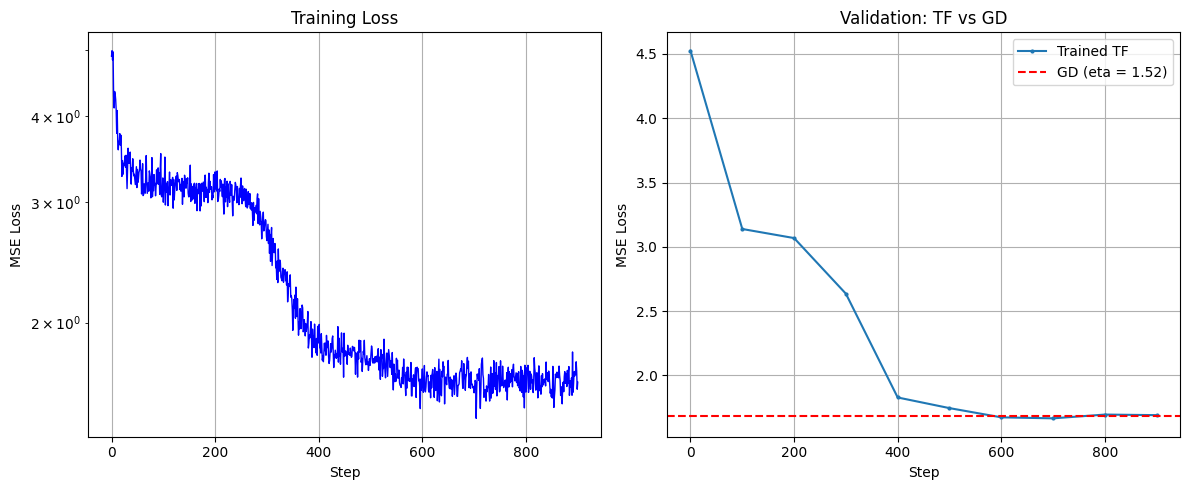
\includegraphics[width=1\textwidth]{LSA-signle-layer-exp, NX=10, NY=1, N=10.png}
    \caption{График сравнения Loss модели и шага GD.}
    \label{fig:loss_comparison}
\end{figure}

\subsubsection{Основной результат}

\textbf{При любых параметрах (они варьировались в дополнительных экспериментах)} (\(n_x, N, w_{\text{std}}\)) обученная модель достигала \textbf{того же loss, что и один шаг GD} с оптимальной \(\eta\). Кривые валидационного loss модели и GD сходились к одному значению.

\subsection{Сходимость матриц к эталонным}

\subsubsection{Случайная инициализация}

При случайной инициализации весов модель \textbf{не сходилась} к эталонным GD-матрицам (\(\cos \approx 0\)). При этом loss модели и GD совпадали. Это объясняется тем, что для линейных сетей без нелинейности существует \textbf{бесконечно много эквивалентных параметризаций}, дающих одинаковый функционал. Авторы статьи также отмечают этот факт в разделе «Uniqueness»:
\begin{quote}
\textit{«The construction is not unique; in particular, it is only required that the products \(PW_V\) as well as \(W_KW_Q\) match the construction. Any rescaling \(s\) of the matrix products leads to an equivalent result.»}
\end{quote}

\subsubsection{Инициализация с возмущением}

При инициализации весов как GD-матрицы + небольшой шум (\(\sigma = 0.01\)) и обучении с малым learning rate (\(10^{-5}\)), матрицы оставались близкими к эталонным (\(\cos > 0.95\)).

\subsection{Эксперименты с замораживанием матриц}

Была проведена серия экспериментов, в которых одна или несколько матриц фиксировались как эталонные GD-матрицы и замораживались, а остальные обучались.

\subsubsection{Заморозка \(W_Q\) или \(W_K\)}

\begin{table}[h]
\centering
\caption{Результаты заморозки \(W_Q\) или \(W_K\)}
\begin{tabular}{@{}lll@{}}
\toprule
Заморожена & Сходимость другой & Косинусное сходство \\
\midrule
\(W_Q\) & \(W_K \to\) GD & \(\pm 0.9\) (за 1000 итераций) \\
\(W_K\) & \(W_Q \to\) GD & \(\pm 0.7\) (за 1000 итераций) \\
\bottomrule
\end{tabular}
\end{table}

\textbf{Результат:} Фиксирование одной из матриц (\(W_Q\) или \(W_K\)) приводит к тому, что другая матрица быстро сходится к эталонной (или к её антиподу с \(\cos \approx -1\)).

\subsubsection{Заморозка \(W_V\) или \(P\)}

\begin{table}[h]
\centering
\caption{Результаты заморозки \(W_V\) или \(P\)}
\begin{tabular}{@{}lll@{}}
\toprule
Заморожена & Сходимость другой & Косинусное сходство \\
\midrule
\(W_V\) & \(W_Q, W_K, P\) далеки от эталонных & -- \\
\(P\) & \(W_Q, W_K\) далеки от эталонных & -- \\
\(P\) & \(W_V \to\) GD & \(\pm 0.4\) \\
\bottomrule
\end{tabular}
\end{table}

\textbf{Результат:} Фиксирование \(W_V\) не приводит к сходимости остальных матриц к эталонным. Фиксирование \(P\) не приводит к сходимости \(W_Q\) и \(W_K\), но при этом \(W_V\) сходится к эталонной с косинусным сходством \(\pm 0.4\).

Модель находит другие решения, функционально эквивалентные GD, но со структурно отличными матрицами.
\subsubsection{Заморозка нескольких матриц}

\begin{table}[h]
\centering
\caption{Результаты заморозки нескольких матриц}
\begin{tabular}{@{}ll@{}}
\toprule
Заморожены & Результат \\
\midrule
\(W_Q\) и \(W_K\) (QK) & \(W_V\) и \(P\) далеки от эталонных \\
\(P\) и \(W_V\) (PV) & \(W_Q\) и \(W_K\) далеки от эталонных \\
\(W_Q, W_K, W_V\) & \(P\) не сошлась к эталонной \\
\(W_Q, W_K, P\) & \(W_V\) сошлась до \(\cos \approx 0.6\) \\
\bottomrule
\end{tabular}
\end{table}

\begin{figure}[h!]
    \centering
    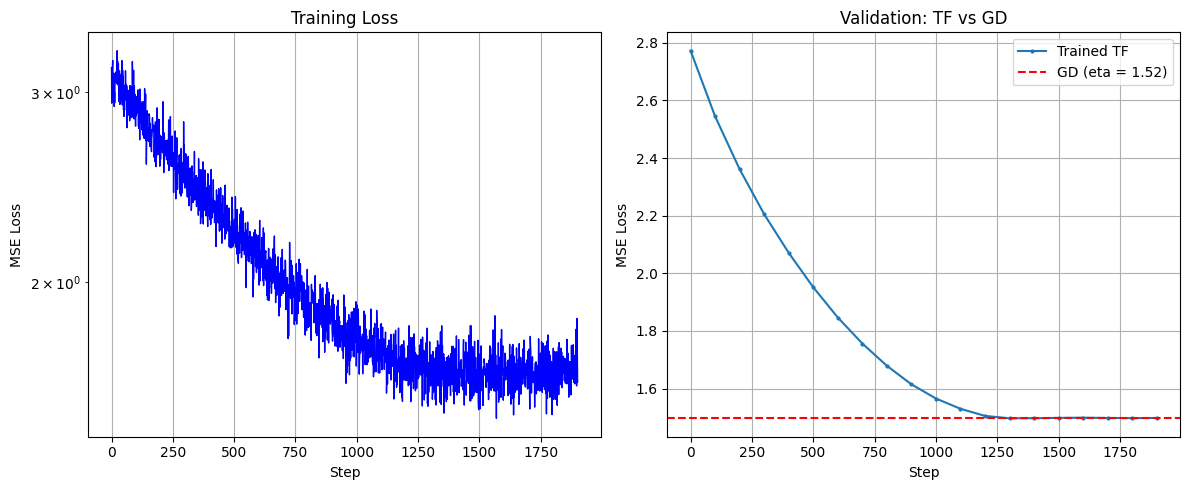
\includegraphics[width=1\textwidth]{LSA-freeze-matrix-exp, QKP.png}
    \caption{График Loss при фиксированных матрицах \(W_Q, W_K, P\)}
    \label{fig:loss_freeze}
\end{figure}

\textbf{Результаты:}
\begin{itemize}
    \item При трёх зафиксированных матрицах \(W_Q, W_K, W_V\) матрица \(P\) не обязательно сходится к эталонной.
    \item При фиксации \(W_Q, W_K, P\) матрица \(W_V\) сходится к эталонной, но медленнее в смысле сходимости к loss (потребовалось на \(\sim 30\%\) больше итераций до достижения GD loss).
\end{itemize}

\subsection{Выводы}

\begin{enumerate}[leftmargin=*]
    \item \textbf{Успешно воспроизведён} основной результат статьи: один слой Linear Self-Attention обучается выполнять один шаг градиентного спуска, достигая того же loss, что и оптимальный GD.

    \item \textbf{Подтверждена неединственность} GD-параметризации: при случайной инициализации модель находит функционально эквивалентные, но структурно отличные матрицы.

    \item \textbf{Эксперименты с замораживанием} показали, что:
    \begin{itemize}
        \item Матрицы \(W_Q\) и \(W_K\) сильно связаны: фиксация одной приводит к сходимости другой к эталонной.
        \item Матрицы \(W_V\) и \(P\) менее «зажаты» — их фиксация не гарантирует сходимости остальных.
        \item Пара \(W_Q, W_K\) является ключевой для определения структуры решения.
        \item Полное восстановление эталонных матриц требует либо инициализации близко к GD, либо регуляризации.
    \end{itemize}
\end{enumerate}

\renewcommand{\refname}{Список литературы}
\begin{thebibliography}{9}

\bibitem{garg2022what}
Garg, S., Tsipras, D., Liang, P. S., \& Valiant, G. (2022). What can transformers learn in-context? A case study of simple function classes. \textit{Advances in Neural Information Processing Systems (NeurIPS)}, 35, 30475-30487.

\bibitem{akyurek2023what}
Akyürek, E., Schuurmans, D., Andreas, J., Ma, T., \& Zhou, D. (2023). What learning algorithm is in-context learning? Investigations with linear models. \textit{International Conference on Learning Representations (ICLR)}.

\bibitem{vonOswald2023}
von Oswald, J., Niklasson, E., Randazzo, E., Sacramento, J., Mordvintsev, A., Zhmoginov, A., \& Vladymyrov, M. (2023). Transformers learn in-context by gradient descent. \textit{International Conference on Machine Learning (ICML)}, PMLR.

\bibitem{gao2024noise}
Gao, H., Zhang, F., Jiang, W., Shu, J., Zheng, F., \& Wei, H. (2024). On the Noise Robustness of In-Context Learning for Text Generation. \textit{Advances in Neural Information Processing Systems (NeurIPS)}.

\bibitem{ahn2023transformers}
Ahn, K., Cheng, X., Daneshmand, H., \& Sra, S. (2023). Transformers learn to implement preconditioned gradient descent for in-context learning. \textit{Advances in Neural Information Processing Systems (NeurIPS)}.

\bibitem{cao2026robust}
Cao, H. T. H., Trinh, H. D. V., Quan, T., \& Truong, L. V. (2026). Transformers Learn Robust In-Context Regression under Distributional Uncertainty. \textit{arXiv preprint arXiv:2603.18564}.

\bibitem{huber1964robust}
Huber, P. J. (1964). Robust estimation of a location parameter. \textit{The Annals of Mathematical Statistics}, 35(1), 73-101.

\end{thebibliography}

\end{document}